\documentclass[letterpaper]{article}

\usepackage[submission]{aaai2027}
\usepackage[hyphens]{url}
\usepackage{microtype}
\usepackage{amsmath}
\usepackage{booktabs}
\usepackage{longtable}
\usepackage{array}
\usepackage{tabularx}
\usepackage{graphicx}
\usepackage{caption}
\usepackage{xcolor}
\usepackage{enumitem}
\usepackage{listings}
\usepackage{rotating}
\usepackage{algorithm}
\usepackage{algpseudocode}
\usepackage[export]{adjustbox}
\urlstyle{rm}
\def\UrlFont{\rm}
\frenchspacing
\emergencystretch=1.2em

\lstdefinestyle{cmd}{
  basicstyle=\ttfamily\scriptsize,
  columns=fullflexible,
  breaklines=true,
  frame=single,
  framerule=0.2pt,
  xleftmargin=0.02\linewidth,
  xrightmargin=0.02\linewidth
}

\newcommand{\weave}{WEAVE}
\newcommand{\dinos}{DINO-S}
\newcommand{\dinoc}{DINO-C}
\newcommand{\clips}{CLIP-S}

\title{Supplementary Material for WEAVE}
\author{Anonymous Submission}
\affiliations{}

\begin{document}
\maketitle

\renewcommand{\thetable}{S\arabic{table}}
\renewcommand{\thefigure}{S\arabic{figure}}
\renewcommand{\thealgorithm}{S\arabic{algorithm}}
\setcounter{table}{0}
\setcounter{figure}{0}
\setcounter{algorithm}{0}

\begin{abstract}
This supplement provides the implementation, evaluation, and diagnostic details needed to
reproduce the main paper. Paths are package-relative. The analytic fiber scale $\beta$ is
an inference-time solver parameter; main-table evaluation uses \texttt{inference.json}
with $\beta{=}2.0$.
\end{abstract}

\section{Reproducibility Overview}

The anonymous archive is a \textbf{minimal code package}: source, configs, and the selected
D5 checkpoint. Datasets, packed latents, and ONNX/TensorRT graphs are \textbf{not}
redistributed in the archive (size limits); they are prepared externally following this
supplement.

\paragraph{Included in the anonymous archive.}
\begin{center}
\footnotesize
\begin{tabularx}{\linewidth}{p{0.48\linewidth}X}
\toprule
Path & Role \\
\midrule
\path{configs/hf_oriented_internal_early_stop.json} & D5 train config (internal early stop). \\
\path{config.json} / \path{inference.json} & Base config; main-table eval override ($\beta{=}2.0$). \\
\path{checkpoints/weave_epoch_0004.pt} & Selected D5 checkpoint. \\
\path{tools/prepare_submission_data.py} & Path sanitize for local data layout. \\
\path{docs/generation_only_timing_summary.json} & Audited 73.0\,s / 750 timing ledger. \\
\path{docs/onnx_export_and_trt.md} & How to export ONNX and compile TensorRT. \\
\path{data/README.md} & Expected local data layout (not the data itself). \\
\bottomrule
\end{tabularx}
\normalsize
\end{center}

\paragraph{Required externally (not in the minimal archive).}
\begin{center}
\footnotesize
\begin{tabularx}{\linewidth}{p{0.48\linewidth}X}
\toprule
Path & Role \\
\midrule
\path{data/train}, \path{data/test} & D5 latents + eval images (build from WikiArt). \\
\path{data/train_p2a}, \path{data/test_p2a}, \path{data/images/r5} & P2A/R5 boards if those rows are re-run. \\
\path{data/onnx_exported/} (optional) & VAE ONNX graphs for the 73\,s timing protocol. \\
Collection-specific P2A/R5 checkpoints & Needed to reproduce those Table~1 rows. \\
\bottomrule
\end{tabularx}
\normalsize
\end{center}

The shipped D5 checkpoint alone does \textbf{not} reproduce the collection-specific P2A or
R5 rows in main-paper Table~1.

\section{Datasets and Evaluation Boards}

\paragraph{D5-512.}
The primary benchmark is Distinct5-WikiArt at 512 px. It contains five WikiArt styles:
Early Renaissance, Impressionism, Minimalism, Rococo, and Ukiyo-e. Training uses 5{,}000
images (1{,}000 per family; the source pool is larger, but a fixed 1{,}000-image subset per
family is used, matching the 52 steps/epoch at batch 96). Evaluation uses all ordered
source-target style pairs with 30 content images per source style, giving 750 pairs. The 150
same-style pairs are retained as identity calibration rows rather than removed.

\paragraph{P2A-256.}
The photo-to-art board evaluates transfer at 256 px. It uses the same ordered evaluation
logic but with a lower-resolution latent/image cache. It is included to test whether the
method remains stable when high-frequency subbands are compressed by resolution.

\paragraph{R5-WikiArt.}
R5 tests collection-specific training on five WikiArt styles drawn at random from WikiArt
and held out from D5: Cubism, Expressionism, Pop Art, Romanticism, and Symbolism
(\path{data/images/r5/test}; 30 images per style). Evaluation uses the same ordered 750-pair
protocol as D5 (\(5\times5\times30\)). Other5 (main-paper zero-shot table) is a different
five-family list held out from D5; it is not required to be disjoint from R5.

\begin{figure}[t]
\centering
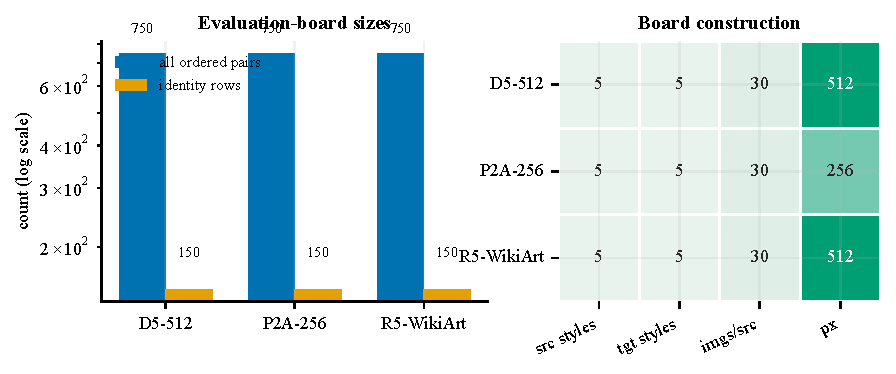
\includegraphics[width=0.88\linewidth]{supplement_figures/fig_dataset_boards.pdf}
\caption{Evaluation-board construction. D5-512, P2A-256, and R5-WikiArt each use a
750-pair board with identity rows retained. R5 is five randomly selected held-out WikiArt
styles (Cubism, Expressionism, Pop Art, Romanticism, Symbolism).}
\label{fig:supp-dataset-boards}
\end{figure}

\paragraph{Pairing and calibration.}
All learned methods use the same ordered pair lists within a board. For D5 training,
source-target pairing uses
\path{data/train/.latent_cache/prototype_pairing_top8.pt} with
\texttt{pairing\_cache\_active\_topk=0}. Identity rows estimate the no-op style floor and
content ceiling.

\subsection{Dataset Layout}

Expected local layout after preparing WikiArt boards (see \path{data/README.md} in the
code package; data themselves are external):

\begin{center}
\footnotesize
\begin{tabularx}{\linewidth}{p{0.42\linewidth}X}
\toprule
Path & Contents \\
\midrule
\path{data/train} & D5 latents + \path{.latent_cache/packed} (train default). \\
\path{data/test} & D5-512 held-out eval images (150). \\
\path{data/train_p2a}, \path{data/test_p2a} & P2A latents and eval images. \\
\path{data/images/d5/train} & D5 train JPGs (optional re-encode). \\
\path{data/images/r5/\{train,test\}} & R5 WikiArt board. \\
\path{data/onnx_exported/} & Optional VAE ONNX graphs (export; not shipped). \\
\bottomrule
\end{tabularx}
\normalsize
\end{center}

\paragraph{Expected counts.}
D5/R5 boards: $5{\times}5{\times}30{=}750$ ordered pairs (identity rows retained).
P2A uses the same ordered-pair protocol at 256\,px; some external baselines provide only
the 600 off-diagonal transfers.

\subsection{Data Preprocessing Contract}

Training consumes latents (VAE scale $0.18215$), not raw RGB. Style directory names must
match the config lists. Pairing caches and metric reference caches are built only from
training latents and held-out test/style-bank images, never from generated outputs.

\section{Hardware and Software Environment}

All training and timing numbers reported in the paper come from a single consumer-class
GPU. The environment is described by role, not by machine identifier:

\begin{center}
\begin{tabularx}{\linewidth}{p{0.38\linewidth}X}
\toprule
Component & Value \\
\midrule
GPU class & NVIDIA GeForce RTX 3060, 12\,GB \\
Training precision & bfloat16 automatic mixed precision \\
TF32 matmul & enabled \\
Device count & 1 GPU \\
\bottomrule
\end{tabularx}
\end{center}

The method itself does not depend on a specific software stack version beyond the ranges listed above; any
consumer GPU with $\geq 12$\,GB VRAM and a working PyTorch CUDA build reproduces the
reported numbers.

The software stack follows \path{WEAVE/requirements.txt}: PyTorch
\(\ge 2.3\), torchvision \(\ge 0.18\), transformers \(4.57 \le v < 5\), diffusers
\(0.38 \le v < 0.39\), LPIPS, torchmetrics, torch-fidelity, Pillow, NumPy, SciPy,
scikit-learn, and tqdm. The frozen VAE is the SD1.5 EMA VAE used only for latent
encoding/decoding; it contributes 84M frozen parameters and is not trained.

\section{Model and Training Setup}

\weave{} trains a compact velocity model in SD1.5 VAE latent space. A single-level Haar
DWT splits the latent into LL/LH/HL/HH subbands. The base network has four residual blocks
of width 64 and three supervised output heads for LL/LH/HL. The D5 model adds separate
pooled target-LH and target-HL encoders whose gated residuals enter only the matching
velocity heads. The complete model has 1,037,087 trainable parameters; the frozen VAE is
reported separately as \(1.04\mathrm{M}^{+84\mathrm{M}}\).

\begin{center}
\begin{tabularx}{\linewidth}{p{0.38\linewidth}X}
\toprule
Field & Paper configuration \\
\midrule
Config & \path{configs/hf_oriented_internal_early_stop.json} \\
Base config & \path{config.json} \\
Seed & 42 \\
Maximum epochs & 15; internal stop at epoch 4 \\
Batch size & 96 \\
Gradient accumulation & 1 \\
Optimizer & AdamW, fused when available \\
Learning rate & \(2.0 \times 10^{-4}\) \\
Minimum learning rate & \(1.0 \times 10^{-5}\) \\
Schedule & cosine \\
Weight decay & \(1.0 \times 10^{-4}\) \\
Gradient clipping & 1.0 \\
Precision & bf16 AMP \\
Channels-last layout & enabled \\
Torch compile & disabled \\
Workers & 0 \\
Checkpoint interval & every epoch \\
Internal probe batch & 4 fixed latents at (t=0.5) \\
\bottomrule
\end{tabularx}
\end{center}

The structure-aligned target is constructed in the wavelet basis. The LL target is a mild
content-preserving blend,
\[
\begin{aligned}
  \mathrm{LL}_{target} ={}&0.7\,\mathrm{LL}_{content} \\
  &+ 0.3\,\mathrm{AdaIN}(\mathrm{LL}_{content}, \mathrm{LL}_{style}),
\end{aligned}
\]
while the high-frequency target uses the target-style LH/HL/HH bands. The implementation
minimizes the band-weighted velocity-matching loss given in the main paper; no additional edge
or low-pass loss is active in the submitted configuration.

\subsection{Resolved Configuration Details}

The frozen merged configuration for the paper run resolves the short public config
into the following relevant fields:

\begin{table*}[t]
\centering
\footnotesize
\begin{tabularx}{\textwidth}{p{0.30\textwidth}p{0.16\textwidth}X}
\toprule
Field & Value & Relevance \\
\midrule
\path{model.contract_family} & \texttt{weave} & Selects the WEAVE architecture contract. \\
\path{model.base_dim} & 64 & Backbone width. \\
\path{model.time_dim} & 256 & Time embedding width. \\
\path{model.num_res_blocks} & 4 & Main residual block count. \\
\path{model.num_hires_blocks} & 2 & High-resolution block count. \\
\path{model.num_decoder_blocks} & 2 & Decoder block count. \\
\path{model.target_latent_hf_subband_fusion_enabled} & true & Activates orientation-specific target-HF residuals. \\
\path{model.target_latent_hf_head_fusion_gate_init} & 0.18 & Initial LH/HL route gate. \\
\path{model.lowpass_mode} & \texttt{dwt\_haar} & Single-level Haar decomposition. \\
\path{model.endpoint_adain_mode} & \texttt{spatial\_fiber} & High-frequency residual statistics matched after every Euler step. \\
\path{model.endpoint_adain_only_last_step} & false & Keeps AdaIN inside all eight integration updates. \\
\path{model.endpoint_adain_scale} & base $1.0$; reported eval $2.0$ & $=\beta$ in the main-paper fiber update $S_s$. $\beta$ affects solver evaluation only and does not enter Eq.~of the main-paper training loss. The base checkpoint stores $1.0$; main Table~1 uses the \texttt{inference.json} override $2.0$, which recovers the reported D5 board means. \\
\path{model.style_extrap_alpha} & 0.1 & $=\eta$: multiplies target HF statistics before matching. \\
\path{bridge.objective_mode} & \texttt{flow\_matching} & Noise-regularized endpoint-velocity regression. \\
\path{bridge.loss_type} & \texttt{mse} & Velocity matching loss. \\
training path & $t\sim\mathcal U[0,1]$ & Time sampling used by the submitted flow objective. \\
\path{bridge.bridge_sigma} & 0.02 & Scales the $\sqrt{t(1-t)}$ interpolation perturbation. \\
\path{bridge.training_target_projection_mode} & \texttt{dwt} & Target construction in wavelet space. \\
\path{bridge.spectral_w_ll/lh/hl/hh} & 0.3/1.0/1.0/inactive & HH has no velocity head in WEAVE. \\
\path{bridge.ll_partial_alpha} & 0.3 & Mild LL style-statistics migration. \\
\path{training.internal_probe_enabled} & true & Measures fixed-batch loss-path gradients after each epoch. \\
\path{training.internal_early_stop_enabled} & true & Stops at the first gate/gradient transition. \\
\bottomrule
\end{tabularx}
\caption{Resolved fields from the frozen paper configuration.}
\label{tab:supp-resolved-config}
\normalsize
\end{table*}

\subsection{Training Log Audit}

The D5 paper run contains four logged epochs, each with 52 optimizer steps and effective
batch size 96. The wall-clock epoch time sums to 82.80 s. The probe is evaluated after the
optimizer and scheduler step, before checkpoint saving, and does not decode images.

\begin{center}
\footnotesize
\setlength{\tabcolsep}{4pt}
\begin{tabular}{@{}rrrrr@{}}
\toprule
Epoch & Loss & Learning rate & Epoch time (s) & Stop event \\
\midrule
1 & 1.3631 & 2.0000e-4 & 25.72 & no \\
2 & 1.3318 & 1.9792e-4 & 19.23 & no \\
3 & 1.3199 & 1.9179e-4 & 18.94 & no \\
4 & 1.2499 & 1.8186e-4 & 18.90 & yes \\
\bottomrule
\end{tabular}
\normalsize
\end{center}

The first epoch is slower because caches and kernels are warmed. Later epochs take about
19 s on a single RTX 3060 (12\,GB), including the fixed-latent probe.

\subsection{Internal-Dynamics Probe}

For a fixed latent minibatch, the implementation performs one backward pass for the LL
loss and one for the summed LH/HL loss. Gradients are aggregated over the shared input,
attention, AdaLN, and feed-forward modules. The target-HF route and ordinary HF heads are
measured separately. The model runs in evaluation mode during the probe, no optimizer step
is taken, and \texttt{torch.random.fork\_rng} restores CPU and CUDA random states.

\begin{center}
\scriptsize
\setlength{\tabcolsep}{2pt}
\begin{tabular}{rrrrrr}
\toprule
Epoch & Gate & $\Delta$Gate & Shared LL/HF & Route/shared & Route/head \\
\midrule
1 & 0.173068 & 0.000000 & 1.4727 & 0.8323 & 0.1816 \\
2 & 0.172264 & -0.000803 & 1.4328 & 0.6133 & 0.1907 \\
3 & 0.172009 & -0.000255 & 1.0868 & 0.4984 & 0.2111 \\
4 & 0.175719 & +0.003710 & 0.1634 & 0.2370 & 0.4561 \\
\bottomrule
\end{tabular}
\normalsize
\end{center}
\captionof{table}{Stopping-trajectory probe on the D5-512 checkpoint (one fixed latent minibatch per epoch).}
\label{tab:supp-stopping-traj}

Epoch 4 is the first joint event where the gate derivative is positive and the shared
LL/HF ratio contracts by at least 35\% from the preceding epoch. A retrospective probe of the complete 15-epoch curve selects
the same epoch, whose DINO-S is the curve maximum. Residual alignment to the FM target,
however, continues to improve after epoch 4 while DINO-S declines. This separates the
proposed transition from ordinary loss-based early stopping: it detects a change in route
ownership rather than a plateau in endpoint regression.

The original absolute crossing-at-one rule was scale-sensitive. Replacing it by
$\rho_e/(\rho_{e-1}+\epsilon)\leq0.65$ selects epoch 4 for probe batches 2/4/8 and seeds
42/7, and epoch 3 for seed 123. The additional seed-7 and seed-123 checkpoints give
(DINO-S, CLIP-S, LPIPS, DINO-C) of (0.4910, 0.7140, 0.2668, 0.8076) and
(0.4862, 0.7144, 0.2552, 0.8040), respectively. Thus the event is stable to the tested
probe scale and keeps the selected point near the canonical frontier; it is not claimed as
an architecture-independent criterion.

\begin{algorithm}[t]
\caption{Evaluation-free internal-dynamics stopping rule}
\label{alg:supp-stopping}
\begin{algorithmic}[1]
\Require trained WEAVE trunk; probe minibatch $\mathcal{B}$; ratio threshold $\tau{=}0.65$; expansion tolerance $\epsilon{>}0$
\State run one LL-loss and one summed LH/HL-loss backward pass on $\mathcal{B}$ (eval mode, no optimizer step)
\State record target-HF gate $g_e$ and shared-trunk LL/HF gradient norm $\rho_e$
\For{$e = 1, 2, \dots$}
  \State compute $\Delta g_e = g_e - g_{e-1}$ and ratio $r_e = \rho_e / (\rho_{e-1} + \epsilon)$
  \If{$\Delta g_e > 0$ \textbf{and} $r_e \le \tau$}
    \State \Return selected epoch $e$ \Comment{first joint gate-expansion \& $\ge 35\%$ LL/HF contraction}
  \EndIf
\EndFor
\Ensure never generate images; never consult DINO-S, CLIP-S, LPIPS, or DINO-C
\end{algorithmic}
\end{algorithm}

\begin{figure}[t]
\centering
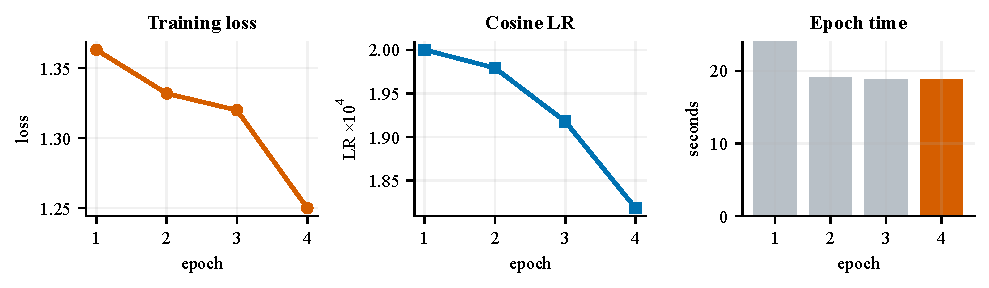
\includegraphics[width=0.9\linewidth]{supplement_figures/fig_training_audit.pdf}
\caption{Training dynamics for the selected D5-512 checkpoint. Training stops at
epoch 4 when the high-frequency conditioning gates increase and the shared LL/HF gradient ratio
contracts sharply relative to the preceding epoch.}
\label{fig:supp-training-audit}
\end{figure}

\subsection{Implementation Notes}

Core modules: \path{run.py}, \path{trainer.py}, \path{internal_dynamics.py},
\path{model.py}, \path{wavelet.py}, \path{utils/run_evaluation.py}. Material details:
VAE scale \texttt{0.18215}; training supervises LL/LH/HL heads (HH via analytic
alignment); evaluation metrics use held-out style-bank caches only.

\section{Information-Flow Diagnosis}

\subsection{Closed-form Pixel--Latent Representability}

We test whether appearance changes that are simple in RGB remain simple after VAE
encoding, without training a network. The test uses 96 source-disjoint requests at
$256{\times}256$ resolution. For each request, we construct four RGB targets: a channel-wise
color shift, AdaIN, WCT, and a channel-wise gamma curve. The target latent is the
deterministic posterior-mean encoding of that same transformed image; posterior sampling is
not used.

In each representation, we independently solve the optimal cross-channel $1{\times}1$
affine map by least squares over all spatial positions of each request. We report its squared
endpoint residual divided by the true endpoint-displacement energy. This normalization makes
zero displacement equal to one in either representation and avoids comparing raw RGB and
latent MSE scales.

\begin{center}
\footnotesize
\setlength{\tabcolsep}{2pt}
\begin{tabular}{lcc}
\toprule
RGB target transformation & Pixel NMSE & VAE-latent NMSE \\
\midrule
Color shift & 0.0072 & 0.2527 \\
AdaIN & 0.0122 & 0.3138 \\
WCT & 0.0143 & 0.3765 \\
Gamma curve & 0.0411 & 0.2937 \\
\bottomrule
\end{tabular}
\end{center}

The small nonzero RGB residuals arise from clipping and, for the gamma target, from its
nonlinearity. The much larger latent residual remains even though the fit is an optimistic
per-request oracle. The result therefore isolates a representation effect: VAE compression
reduces spatial computation, but a pointwise RGB appearance change need not remain pointwise
or affine in latent coordinates.

As a matched nonlinear check, we train the same four-layer $1{\times}1$ conditional MLP in
both representations for 1,500 optimizer steps and three seeds. Both versions use width 64,
SiLU activations, identical request batches and sampled spatial positions, and the same RGB
content/style means and standard deviations as conditioning. This is a separate pointwise
representation diagnostic, not an image-quality evaluation.

\begin{center}
\footnotesize
\begin{tabular}{lc}
\toprule
Representation & Endpoint NMSE \\
\midrule
Pixel & $0.0327\pm0.0004$ \\
VAE latent & $0.3126\pm0.0041$ \\
\bottomrule
\end{tabular}
\end{center}

The latent curve plateaus near its closed-form affine residual, whereas Pixel continues
toward the target.

Main-paper Figure~4(b) uses a spatial TinyUNet with approximately 7.6M parameters, 480 training pairs,
30 epochs, and three seeds. All variants use the same global velocity MSE. Pixel and plain
latent transport use the RGB-AdaIN endpoint in their respective representations; the third
variant changes only the latent endpoint to LL from the source and LH/HL/HH from the style.

\begin{center}
\footnotesize
\setlength{\tabcolsep}{4pt}
\begin{tabular}{@{}lcc@{}}
\toprule
Transport setting & Final NMSE & Seeds \\
\midrule
Pixel, RGB-AdaIN endpoint & $0.0418\pm0.0029$ & 3 \\
VAE latent, RGB-AdaIN endpoint & $0.3542\pm0.0060$ & 3 \\
VAE latent, spectral endpoint & $0.0086\pm0.0004$ & 3 \\
\bottomrule
\end{tabular}
\end{center}

The frequency-decoupled endpoint is substantially easier for the same network to regress.
This is an internal learnability result, not an external image-quality comparison.

\subsection{Latent Subband Statistics}

We apply one-level orthonormal Haar decomposition to 5,000 deterministic SD1.5 EMA-VAE
latents from five Distinct5 styles. For each latent, subband energy is normalized by total
latent energy. Style separability uses 500 latents (100 per style): the scalar response is
the per-image mean absolute coefficient in each band, and the reported $\eta^2$ is the
one-way ANOVA effect size of the style label.

\begin{center}
\footnotesize
\begin{tabular}{lrrrr}
\toprule
Band & Mean energy & p5 & p95 & Style $\eta^2$ \\
\midrule
LL & 0.659 & 0.459 & 0.904 & 0.436 \\
LH & 0.115 & 0.032 & 0.184 & 0.270 \\
HL & 0.125 & 0.038 & 0.201 & 0.375 \\
HH & 0.101 & 0.021 & 0.171 & 0.499 \\
\bottomrule
\end{tabular}
\end{center}

Because Haar is orthonormal, the energy shares are directly comparable and sum to one.
They show a clear scale imbalance rather than an extreme low-pass collapse. The ANOVA result
also rejects a hard semantic assignment of LL to content and HH to style: every band is
style-sensitive, with a non-monotonic orientation pattern and the largest effect in HH.
These measurements motivate separate frequency routes and partial LL movement; they do not
determine the numerical LL blend or loss weight, which are evaluated by ablation.

\paragraph{Terminal frequency dynamics.}
We also evaluate matched 10-epoch checkpoints with $\lambda_{LL}=0.3$ and $1.0$ on the same
fixed batch of four cross-style pairs at $t=0.5$ (seed 42). The values below are a terminal
internal snapshot, not an average over training.

\begin{center}
\footnotesize
\begin{tabular}{lrrrr}
\toprule
$\lambda_{LL}$ & LL loss & HF loss & $\|g_{LL}\|_2$ & $\|g_{HF}\|_2$ \\
\midrule
0.3 & $3.03\!\times\!10^{-2}$ & 1.144 & 0.592 & 1.611 \\
1.0 & $2.94\!\times\!10^{-8}$ & 1.144 & $4.27\!\times\!10^{-7}$ & 2.113 \\
\bottomrule
\end{tabular}
\end{center}

Uniform weighting reaches a nearly zero LL residual and LL gradient while its HF state is
essentially unchanged. The weighted model retains active gradients in both routes. This
supports monitoring and weighting bands separately, but a single terminal batch does not by
itself identify parameter capacity as the cause.

\begin{figure}[t]
\centering
\includegraphics[width=0.9\columnwidth]{fig_fiber_path_diagnostics.png}
\caption{Per-step routed motion over eight cross-style probes. $S_s$ supplies the dominant HF update, while analytic LL leakage remains below $3.2\times10^{-6}$.}
\label{fig:supp-fiber-path}
\end{figure}

\paragraph{Boundary of the HH-path diagnostic.}
Across 50 cross-style pairs, the directly comparable output correlations are
$0.0245\mathbin{\pm}0.0108$ for an HH-head reconstruction and
$0.0238\mathbin{\pm}0.0115$ for AdaIN; magnitude correlations are respectively
$0.0316\mathbin{\pm}0.0119$ and $0.0294\mathbin{\pm}0.0137$. Thus this test finds no
meaningful increase in output-level target topology from the HH head. Its velocity correlates
with the supervised HH displacement ($0.2086\mathbin{\pm}0.1275$), but AdaIN has no
corresponding velocity variable, so these quantities should not be divided into a leakage
factor. We therefore treat the HH-head choice as the style--content trade-off reported by the
ablation, not as evidence of inevitable geometric leakage.

The probe campaign was designed to answer a narrower question than the main table:
whether the model's weak style movement came from a wrong target, insufficient training
time, or a disconnected conditioning path. The diagnosis favors the third explanation.
The structure-aligned target already asks for style in the high-frequency bands:
\begingroup
\small
\[
\begin{aligned}
\mathrm{LL}_{target}={}&0.7\,\mathrm{LL}_{content} \\
  &+0.3\,\mathrm{AdaIN}(\mathrm{LL}_{content},\mathrm{LL}_{style}),\\
\mathrm{LH/HL/HH}_{target}={}&\mathrm{LH/HL/HH}_{style}.
\end{aligned}
\]
\endgroup
Thus the loss is not merely reconstructing the source image. The failure mode is that,
in the baseline, the target image latent is used to construct supervision but does not
strongly enter the velocity predictor as an image-specific condition.

\begin{center}
\footnotesize
\begin{tabularx}{\linewidth}{p{0.26\linewidth}p{0.30\linewidth}X}
\toprule
Route & Signal path & Probe reading \\
\midrule
Baseline style memory & \texttt{style\_id} \(\rightarrow\) style memory \(\rightarrow\) cross-attention & Coarse style prior. Gates stay near 0.056--0.061, but removing this route hurts full metrics, so it is useful but not sufficient. \\
Global target-token fusion & target latent \(\rightarrow\) all style tokens \(\rightarrow\) backbone & Connected but too global; it over-controls LL and does not improve useful style transfer. \\
Raw spatial target-HF & target DWT-HF maps \(\rightarrow\) HF residual maps & Has sufficient capacity, but leaks target geometry and collapses content. \\
Pooled subband target-HF & target DWT-HF \(\rightarrow\) per-subband pooled code \(\rightarrow\) HF residual velocity & Current usable path: stronger style signal without target-coordinate leakage. \\
\bottomrule
\end{tabularx}
\normalsize
\end{center}

The strongest negative control is the raw spatial target-HF route. It raises \dinos{}
and \clips{}, which shows that the network can read target-style information when the
path is opened. However, the same run reduces \dinoc{} to 0.4043 and raises LPIPS to
0.5382, so the gain is not a valid style-transfer improvement. It is target-layout
leakage. The accepted route therefore compresses target high frequencies into
coordinate-free subband codes before they reach the HF velocity heads.

\subsection{Probe Protocol and Result Ledger}

Diagnostic target-HF probes fine-tune from a shared base checkpoint and evaluate on D5.
The main accepted lessons are:

\begin{itemize}[leftmargin=1.5em,itemsep=0.2em]
  \item Spatial target-HF injection can raise style scores but leaks target geometry
  (DINO-C collapses; LPIPS rises sharply) and is rejected.
  \item Coordinate-free pooled/subband target-HF codes preserve content while retaining
  most of the style gain; this is the route used by the paper D5 model.
  \item Zeroing subband residuals at inference lowers both style and content metrics, so
  the learned residual path is active rather than dead weight.
  \item Scalar residual amplification, time-windowing, FiLM heads, and memory-prior
  subtraction do not improve the balanced operating point over the simple subband code.
  \item Style memory is a useful coarse prior: removing it weakens transfer, but it cannot
  replace image-specific HF codes.
\end{itemize}

Representative board means (DINO-S / DINO-C / LPIPS / CLIP-S): spatial 0.490/0.404/0.538/0.748
(reject); subband 0.489/0.798/0.297/0.721 (accepted family); residual ablated 0.486/0.789/0.301/0.721.

\section{Inference Setup}

The main paper uses an 8-step Euler solver. Spatial-fiber AdaIN is applied to the
high-frequency residual after every solver step. The main D5-512 row uses
\path{runs/submission/canonical_oriented_epoch4/epoch_0004.pt} (oriented target-HF
route). P2A and R5 use audited base-WEAVE checkpoints with the same Haar endpoint and
stepwise-alignment formulation but without the later oriented D5 route.

\begin{center}
\footnotesize
\begin{tabularx}{\linewidth}{p{0.42\linewidth}X}
\toprule
Inference field & Value \\
\midrule
ODE solver & Euler \\
ODE steps & 8 \\
Generation batch size & 8 (ONNX/TRT pipeline; encoder$+$WEAVE fused stage) \\
VAE encode backend & ONNX Runtime FP16 (\texttt{encoder\_b8.onnx}) \\
VAE decode backend & TensorRT FP16, workspace 2\,GB (\texttt{decoder\_b8.onnx}) \\
Spatial-fiber AdaIN & every Euler step; main-table eval uses \texttt{endpoint\_adain\_scale}${}={}$2.0 via \texttt{inference.json} ($\beta$ in the main paper; train uses $1.0$) \\
Style extrapolation & $\eta=\texttt{style\_extrap\_alpha}=0.1$ \\
Generated-image count for timing & 750 \\
Timing column & end-to-end generation wall clock (encode $+$ ODE $+$ decode; metrics excluded) \\
\bottomrule
\end{tabularx}
\normalsize
\end{center}

\subsection{Evaluation Runtime Anatomy}

The paper reports the measured generation-only time for the selected D5 checkpoint:
73.0\,s for 750 images (97.3\,ms/image) on one RTX 3060 (12\,GB) under the audited
ONNX/TRT pipeline (batch 8, decoder workspace 2\,GB). Stage breakdown:
encoder$+$WEAVE 14.0\,s (18.7\,ms/image, 19\%), TRT decoder 59.0\,s (78.6\,ms/image,
81\%). The timing includes the 8-step trajectory and VAE encode/decode, but excludes
latent caching, metric extraction, and result serialization. Larger decode batch (16)
triggers TRT build OOM on a 12\,GB card and is not used. Increasing decoder workspace
from 2\,GB to 4\,GB improves decode by only $\approx\!0.6\%$ and is not required.
The latent cache itself is a one-time offline VAE encode of the full D5 training set
($5{,}000$ images at $512^{2}$); with our fixed encoder-only ONNX graph under TensorRT
($\approx\!37$\,ms/image) this takes about $3$ minutes, and is amortized across all runs
that reuse the same packed cache.

\begin{figure}[t]
\centering
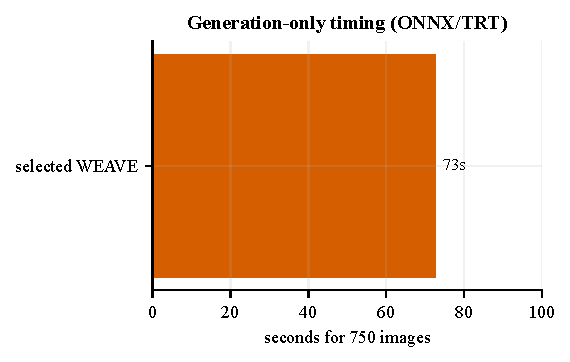
\includegraphics[width=0.56\linewidth]{supplement_figures/fig_timing_breakdown.pdf}
\caption{Generation-only time for the selected WEAVE checkpoint on a single RTX 3060
(12\,GB): 73.0\,s for 750 images (97.3\,ms/image; ONNX/TRT pipeline). Latent caching and
metric computation are excluded.}
\label{fig:supp-timing}
\end{figure}

\subsection{Inference Variants}

The following older base-WEAVE variants share one checkpoint and differ only in
inference-time stepwise AdaIN strength. They remain diagnostic operating points and are
not the updated main D5 result.

\begin{table*}[t]
\centering
\footnotesize
\begin{tabularx}{\textwidth}{lrrrrX}
\toprule
Variant & Scale & \dinos{} & \clips{} & LPIPS & Use \\
\midrule
\texttt{WEAVE-m} & 1.5 & 0.4843 & 0.7180 & 0.2925 & Balanced diagnostic point. \\
\texttt{WEAVE-s} & 1.6 & 0.4845 & 0.7179 & 0.2867 & Peak average of DINO-S and CLIP-S. \\
\texttt{WEAVE-q} & 2.0 & 0.4859 & 0.7075 & 0.2583 & Previous base-WEAVE max-DINO diagnostic. \\
\bottomrule
\end{tabularx}
\caption{Alternative inference settings evaluated from the same base checkpoint.}
\label{tab:supp-inference-variants}
\end{table*}

The audited generation-only timing for the selected checkpoint on a single RTX 3060
(12\,GB; batch 8; TRT decoder workspace 2\,GB) is:

\begin{center}
\begin{tabular}{lr}
\toprule
Timing field & Value \\
\midrule
Total generation-only wall clock & 73.0 s \\
Encoder$+$WEAVE stage & 14.0 s (18.7 ms/img) \\
TRT decoder stage & 59.0 s (78.6 ms/img) \\
Images & 750 \\
Wall time per image & 97.3 ms \\
Throughput & 10.3 pairs/s \\
\bottomrule
\end{tabular}
\end{center}

\section{Metrics}

\paragraph{\dinos.}
\dinos{} is the primary style metric. It is the cosine similarity between the DINOv2-small
CLS feature of the generated image and the nearest reference feature in the target-style
reference pool. The source image is excluded from the reference pool when applicable.

\paragraph{\clips.}
\clips{} is the secondary style metric, computed as CLIP ViT-B/32 image-feature cosine
similarity to the target-style reference prototype.

\paragraph{\dinoc.}
\dinoc{} measures content preservation as DINOv2-small CLS cosine similarity between the
generated image and the source image.

\paragraph{LPIPS.}
LPIPS uses the AlexNet backbone and is reported as a lower-is-better content distance.
Radar plots display \(1-\mathrm{LPIPS}\) so all axes point outward for better values.

\subsection{IDT--TGT Evaluation Guideline}

The guideline adds two source-independent reference outputs to the ordinary metric table.
For a request with source image $x$ and target style $s$, define
\begin{equation}
  y_{\mathrm{IDT}}(x,s)=x,
  \qquad
  y_{\mathrm{TGT}}(x,s)=r_s,
\end{equation}
where $r_s$ is a fixed image from the held-out reference pool for style $s$. The D5
implementation selects the first image in the deterministic reference order and reuses it
for every source paired with that target style. Thus TGT depends on the requested style but
not on source content. It is an evaluation control, not an input to \weave{} or any baseline.

\paragraph{Why two references are needed.}
IDT represents a no-op: it preserves all source content but makes no requested edit. A
method should therefore score above IDT on \dinos{} and \clips{} before a low LPIPS can be
read as successful transfer. TGT represents the opposite extreme: it has the requested
style but unrelated content. A content-preserving method should have lower LPIPS and higher
\dinoc{} than TGT. The intuitive acceptable region is therefore bracketed by
\begin{equation}
\begin{aligned}
M_{\mathrm{style}}(y)&>M_{\mathrm{style}}(y_{\mathrm{IDT}}),\\
\mathrm{LPIPS}(y,x)&<\mathrm{LPIPS}(y_{\mathrm{TGT}},x),\\
\mathrm{DINO\text{-}C}(y,x)&>\mathrm{DINO\text{-}C}(y_{\mathrm{TGT}},x).
\end{aligned}
\end{equation}
We inspect the inequalities separately and do not combine them into a weighted score.

\paragraph{Interpretation and scope.}
IDT and TGT are empirical anchors, not mathematical bounds: a generated image may score
outside either reference because the metrics are imperfect. Crossing IDT in the wrong
direction indicates style suppression under that metric. Moving beyond TGT in content
distance identifies a content-loss regime relative to a deliberately unrelated target-style
image. This is a prompt for visual inspection, not a verdict on the method outside the
current board and metric. On D5-512, IDT
is (\dinos{} 0.419, \clips{} 0.640, LPIPS 0, \dinoc{} 1), while TGT is
(1.000, 0.855, 0.756, 0.220). TGT reaches \dinos{} 1.000 because the selected reference is
part of the same target-style feature pool used by that metric; this value is expected and
should not be read as model performance.

Using each of the first five deterministic target exemplars changes TGT LPIPS from 0.752
to 0.783 and \dinoc{} from 0.189 to 0.246. StyleAligned remains beyond every TGT LPIPS
anchor (0.869), so the content-collapse diagnosis is not determined by the first exemplar.

\subsection{Metric Cache and Determinism}

Evaluation uses deterministic seeds and cached reference features. Cache entries are
logical artifacts under \path{<CACHE_ROOT>/eval_cache}; they may be rebuilt as long as
the image roots and model backbones are unchanged. The full-eval summaries record:
\begin{itemize}[leftmargin=1.5em,itemsep=0.2em]
  \item CLIP backend: HuggingFace transformers backend.
  \item LPIPS network: AlexNet.
  \item Reference-cache limit per style: 16 for the paper full-eval records.
  \item Source-feature cache: one cache per board/image-size setting.
  \item Metric postprocessing: disabled for the main records.
\end{itemize}

\subsection{DINO Sidecar Coverage}

The DINO sidecar contains 37 board-method entries. D5-512 and P2A-256 each include 13
methods: Identity, SD-Turbo, StyleAligned, Z-STAR, StyleShot, CUT, SaMST, SaMam,
Seedream 4.5, Latent-WCT/WCT, StyleID, AdaIN, and \weave{} as applicable. R5-WikiArt
contains 11 entries because not every diagnostic baseline was rerun on the R5 board.
The paper table is manually aligned to these sidecars and the CLIP/LPIPS summaries.

\paragraph{Metric interpretation caveats.}
\dinos{} and \clips{} are style-reference similarities, not human preference labels.
\dinoc{} and LPIPS quantify source preservation, but they penalize different failure
modes: LPIPS is sensitive to perceptual pixel/feature distance, whereas \dinoc{} is a
semantic feature similarity. The paper therefore treats the result as a multi-objective
operating point. A method with high \dinos{} and very high LPIPS is not considered a
content-preserving transfer method even if it appears strong on style alone.

\section{Main Results Used by the Paper}

The complete multi-method ledgers for D5-512, P2A-256, and R5-WikiArt appear in the main
paper Table~1; we do not restate those rows here. For convenience, the \weave{} board means
used by the paper are:

\begin{center}
\small
\setlength{\tabcolsep}{5pt}
\begin{tabular}{@{}lrrrr@{}}
\toprule
Board & \dinos{} & \clips{} & LPIPS & \dinoc{} \\
\midrule
D5-512 & 0.4916 & 0.7128 & 0.2593 & 0.8103 \\
P2A-256 & 0.4801 & 0.6681 & 0.3116 & 0.8612 \\
R5-WikiArt & 0.5226 & 0.7747 & 0.2895 & 0.7717 \\
\bottomrule
\end{tabular}
\normalsize
\end{center}

\begin{figure*}[t]
\centering
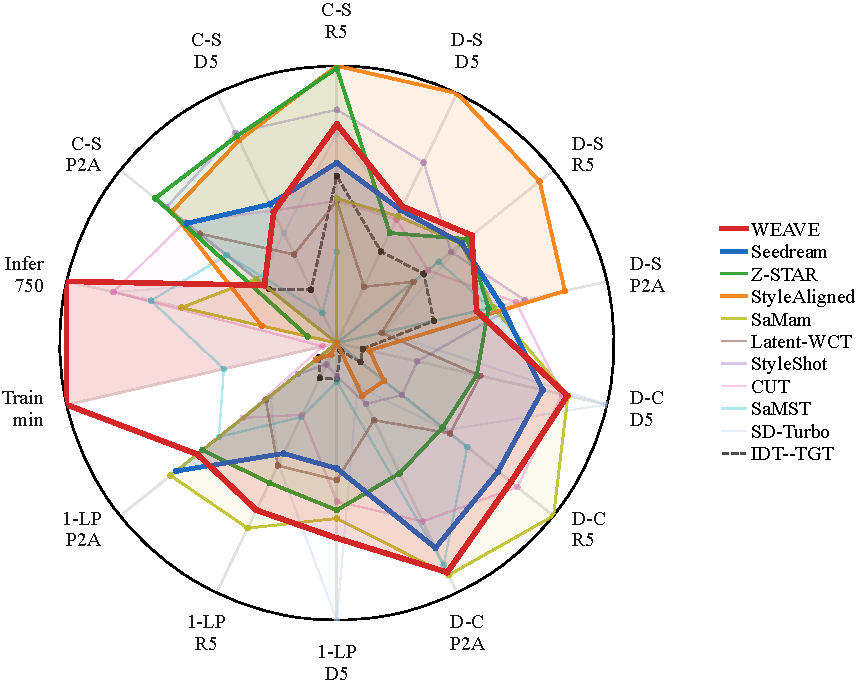
\includegraphics[width=0.9\textwidth]{supplement_figures/fig_radar_full.pdf}
\caption{Style, content, and cost across three benchmarks. The dashed boundary uses
IDT on style axes and TGT on content axes. Each metric family is min--max normalized
once across all reported methods and datasets; speed uses the same normalization after
$\log_{10}(1+t)$, where $t$ is seconds. Raw values are those of main-paper Table~1.}
\label{fig:supp-radar}
\end{figure*}

\begin{figure}[t]
\centering
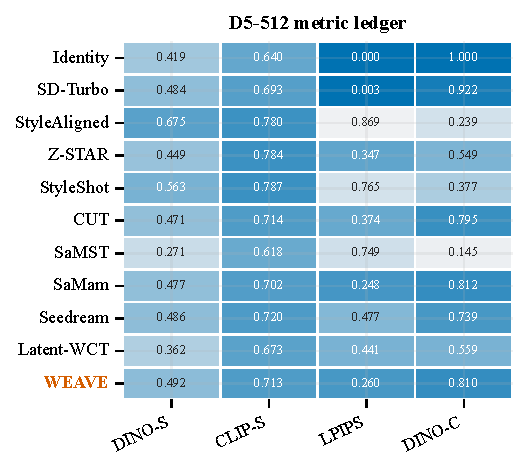
\includegraphics[width=\linewidth]{supplement_figures/fig_d5_metric_heatmap.pdf}
\caption{D5-512 metric ledger as a heatmap. LPIPS cells are color-normalized after
inversion for readability, while annotations show raw values from main-paper Table~1.}
\label{fig:supp-d5-heatmap}
\end{figure}

The D5-512 claim is a balanced Pareto claim rather than a winner-on-every-axis claim:
StyleAligned reaches higher raw \dinos{} but with severe content loss, while \weave{}
keeps low LPIPS, high \dinoc{}, about one million trainable parameters, and a 1.4-minute
training time on one RTX 3060. The D5 point uses the oriented route; the other boards retain
the base model, as stated in the main-table caption.

\begin{figure}[t]
\centering
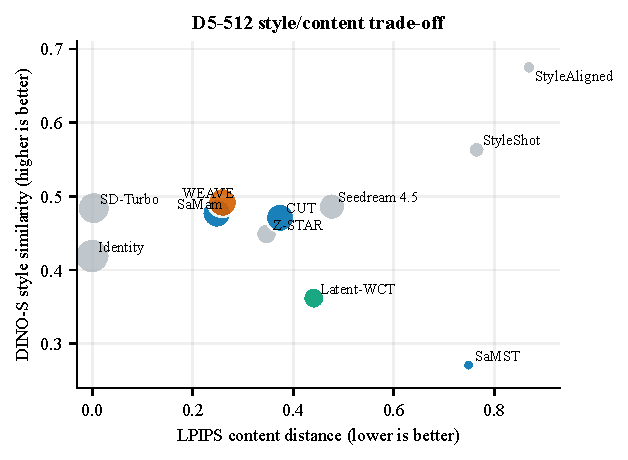
\includegraphics[width=0.6\linewidth]{supplement_figures/fig_d5_tradeoff.pdf}
\caption{D5-512 style/content trade-off. Marker size grows with \dinoc{}. WEAVE is not
the maximum-style point, but it occupies the low-LPIPS, high-content region among learned
methods that clear the identity style floor.}
\label{fig:supp-d5-tradeoff}
\end{figure}

\subsection{Paired Significance Tests on D5}
\label{sec:supp-sig}

The main paper reports mean metrics only. Using the same per-sample metric CSVs that
underlie main-paper Table~1, we run a two-sided paired $t$-test on each metric
($n{=}750$ except Seedream $n{=}720$). Table~\ref{tab:supp-sig} reports
$\Delta=\text{WEAVE}-\text{baseline}$; positive $\Delta$ is better for DINO-S/CLIP-S/DINO-C
and worse for LPIPS. Against our SaMam retrain (CLIP-S $0.702$, LPIPS $0.248$), WEAVE has
significantly higher DINO-S and CLIP-S with statistically indistinguishable content metrics
under this pairing; relative to StyTR-2, AesPA-Net, and Seedream, WEAVE trades style for
content, consistent with the main operating point.

\begin{table}[t]
\centering
\small
\renewcommand{\arraystretch}{0.95}
\setlength{\tabcolsep}{3pt}
\begin{tabular}{@{}lcccc@{}}
\toprule
Baseline & DINO-S & CLIP-S & LPIPS & DINO-C \\
\midrule
CUT        & $+0.012^{***}$ & $+0.012^{***}$ & $-0.072^{***}$ & $-0.006$\,ns \\
StyTR-2    & $-0.018^{***}$ & $-0.004$\,ns   & $-0.359^{***}$ & $+0.042^{***}$ \\
AesPA-Net  & $-0.037^{***}$ & $-0.019^{***}$ & $-0.311^{***}$ & $+0.188^{***}$ \\
SaMam      & $+0.014^{***}$ & $+0.007^{***}$ & $+0.006$\,ns   & $-0.002$\,ns \\
Seedream 4.5 & $-0.008^{*}$ & $-0.014^{***}$ & $-0.153^{***}$ & $+0.049^{***}$ \\
\bottomrule
\end{tabular}
\caption{Paired $t$-test on D5: mean difference $\Delta=$ WEAVE $-$ baseline from the
same per-sample metric CSVs as main-paper Table~1 (SaMam CLIP-S $0.702$, LPIPS $0.248$).
Positive $\Delta$ is better for DINO-S/CLIP-S/DINO-C, worse for LPIPS.
$^{***}$: $p<0.001$; $^{**}$: $p<0.01$; $^{*}$: $p<0.05$; ns: not significant.
CUT/StyTR-2/AesPA-Net/SaMam use $750$ pairs; Seedream uses $720$ overlapping pairs.}
\label{tab:supp-sig}
\end{table}

\subsection{Memory-Only Style Registration}
\label{sec:supp-register}

This section details the registration experiment reported in the main paper
(Memory-only style registration, Generalization and Robustness).

\paragraph{Registration split.}
Registration uses the held-out WikiArt registration split: the five Other5 families
(Abstract Expressionism, Art Nouveau / Modern, Cubism, Expressionism, Symbolism), each of
which is held out from the D5 collection. For each family we draw 30 registration images and
30 evaluation images from disjoint pools; the 30 evaluation images per style form the same
750-pair Other5 board used for the zero-shot comparison (Table~4, main paper). The
registration and evaluation image lists per family are included in the anonymous package.

\paragraph{Optimization.}
Starting from the trained D5 seed-42 checkpoint, we append five new memory entries (one bank
of $256\times384$ tokens per family) and freeze all existing parameters: the velocity trunk,
the LL/LH/HL routed heads, the frozen VAE, the analytic operator, and the five existing D5
memory entries. New entries are initialized with $0.02\cdot\mathcal N(0,I)$, matching the
style-memory initialization scale used during D5 training. Optimization uses AdamW
(learning rate $2\times10^{-4}$, weight decay $10^{-4}$) with the same flow-matching objective
as training, for a fixed 3{,}000-step budget with no evaluation-metric checkpoint selection.
Memory-only registration uses batch size 4 and optimizes only the appended entries (0.098M
parameters per family, 0.49M total); full-field fine-tuning uses batch size 2 and optimizes
all 1.53M parameters of the expanded model. Both variants start from the same appended-memory
initialization and use identical registration data and the same inference configuration
($\beta{=}2.0$, $\eta{=}0.1$, $K{=}8$). Stochasticity is limited to the memory initialization
and minibatch sampling.

\paragraph{Timing.}
Memory-only registration of all five families takes approximately 98\,s
(3{,}000 steps, batch 4); full-field fine-tuning takes approximately 4\,min (3{,}000 steps,
batch 2). Both are measured on the same single RTX~3060 (12\,GB) used for D5 training; the
timing excludes the one-time offline VAE encode of the registration images. Evaluation reuses
the same DINOv2-small protocol as Table~4.

\paragraph{Per-style breakdown.}
Table~\ref{tab:supp-register-perstyle} reports memory-only registration metrics per target
family (150 pairs each). All five families exceed the aggregate zero-shot DINO-S of 0.531,
so the overall gain is not driven by a single style.

\begin{table}[t]
\centering
\small
\setlength{\tabcolsep}{4pt}
\begin{tabular}{@{}lcccc@{}}
\toprule
Target family & DINO-S$\uparrow$ & CLIP-S$\uparrow$ & LPIPS$\downarrow$ & DINO-C$\uparrow$ \\
\midrule
Abstract Expressionism & 0.546 & 0.798 & 0.264 & 0.822 \\
Art Nouveau / Modern   & 0.551 & 0.763 & 0.261 & 0.810 \\
Cubism                 & 0.557 & 0.786 & 0.275 & 0.792 \\
Expressionism          & 0.573 & 0.788 & 0.256 & 0.832 \\
Symbolism              & 0.584 & 0.784 & 0.268 & 0.804 \\
\midrule
All (750 pairs)        & 0.562 & 0.784 & 0.265 & 0.812 \\
\bottomrule
\end{tabular}
\caption{Per-target-family breakdown of memory-only registration on the 750-pair Other5
board (150 pairs per family, including the same-style diagonal). Every family clears the
aggregate zero-shot DINO-S of 0.531.}
\label{tab:supp-register-perstyle}
\end{table}

\paragraph{No forgetting on registered D5 styles.}
Registration freezes the D5 trunk, routed heads, analytic operator, and the five existing D5
memory entries, and appends new entries at higher indices; the D5 forward path therefore does
not read the new entries. Consequently, registering Other5 leaves the D5 outputs unchanged up
to numerical determinism, and no re-evaluation of the D5 board is required to establish
no-forgetting.

\paragraph{Registration image-count curve.}
To probe the data requirement of registration, we vary the number of registration images
per family $n\in\{1,5,10,30\}$ (nested subsets of the 30-image pool) while keeping the fixed
3{,}000-step memory-only budget and all other settings, and evaluate on the same 750-pair board.
Quality is already saturated at a single reference image: DINO-S rises from 0.558 at $n{=}1$
to 0.562 at $n{=}30$ (a gain of only 0.004), and CLIP-S, LPIPS, and DINO-C stay within their
$n{=}30$ values throughout (Table~\ref{tab:supp-register-imgcount}). Registration wall-clock is
essentially independent of $n$ because the 3{,}000-step budget dominates; on our hardware it
varies only between 60\,s and 105\,s across $n{=}1\ldots30$ (the RTX~3060 timing above reports
$\approx$98\,s for $n{=}30$). Together these show that registering a new style is a low-burden
operation: supplying more reference images barely changes the cost yet yields negligible further
gain beyond the first image.

\begin{table}[t]
\centering
\small
\setlength{\tabcolsep}{4pt}
\begin{tabular}{@{}ccccccc@{}}
\toprule
$n$ & DINO-S$\uparrow$ (all/off) & CLIP-S$\uparrow$ & LPIPS$\downarrow$ & DINO-C$\uparrow$ & Time (s) \\
\midrule
1  & 0.558 / 0.492 & 0.782 & 0.260 & 0.820 & 60  \\
5  & 0.561 / 0.498 & 0.784 & 0.269 & 0.812 & 101 \\
10 & 0.561 / 0.498 & 0.784 & 0.270 & 0.808 & 102 \\
30 & 0.562 / 0.499 & 0.784 & 0.266 & 0.813 & 105 \\
\bottomrule
\end{tabular}
\caption{Registration image-count curve on the 750-pair Other5 board. Each row registers the five
Other5 families from the D5 checkpoint using $n$ registration images per family (nested subsets of
the 30-image pool) and a fixed 3{,}000-step memory-only budget. DINO-S is reported over all 750
pairs and the 600 off-diagonal pairs. Quality is saturated at a single reference image, and
registration time is essentially independent of $n$.}
\label{tab:supp-register-imgcount}
\end{table}

\subsection{Hyperparameter Sensitivity}
\label{sec:supp-hypersens}

This section reports one-factor sweeps of the solver-step count $K$ and the inference-time
analytic alignment strength $\beta$ and style-extrapolation $\eta$ on the D5-750 board. The
headline finding is that WEAVE is stable over $K\in\{2,4,8,16\}$ and
$\beta\in[1,2]$ (CLIP-S varies by $<0.001$ across $K$; the style--content trade-off is
preserved throughout $\beta\in[1,2]$), while $\beta\ge2.5$ collapses content and larger
$\eta$ shifts the operating point toward content preservation. $\beta{=}2.0$, $\eta{=}0.1$,
$K{=}8$ is the reported operating point; no D5-test-board search reselects it.

Unless noted, sweeps use the D5-750 board and seed~42. Training-time parameters
($\alpha$, $\lambda_{LL}$) retrain with the same evaluation-free stopping rule when
applicable. Inference-time parameters reuse a fixed checkpoint and vary only the listed knob.
In the solver implementation,
$\mathrm{HF}\leftarrow(1-\beta)\mathrm{HF}+\beta\,\mathcal A(\mathrm{HF};(1+\eta)q_s)$ with
$\beta=\texttt{endpoint\_adain\_scale}$ and $\eta=\texttt{style\_extrap\_alpha}$. Training
defaults are $\alpha{=}0.3$, $\lambda_{LL}{=}0.3$, and $\sigma{=}0.02$. Main-table
evaluation uses $\beta{=}2.0$, $\eta{=}0.1$, $K{=}8$ via \texttt{inference.json}
($\beta$ is solver-only and does not enter the training loss). One-factor diagnostic
sweeps below (including other $\beta$ settings) illustrate
trade-offs and stability boundaries; where a default row does not exactly match the oriented
main-table metrics, the trend---not the absolute score---is the intended takeaway, and no
D5-test-board search reselects the main-row config.

\paragraph{Source-alignment strength $\alpha$.}
Table~\ref{tab:supp-alpha} and Figure~\ref{fig:supp-sens-alpha} vary
$\tilde\ell_s=(1-\alpha)\ell_c+\alpha\,\mathrm{AdaIN}(\ell_c,\ell_s)$.
The method remains stable over $\alpha\in[0.2,0.5]$, with $\alpha{=}0.3$ providing the
strongest style affinity among the scanned settings while retaining low LPIPS.

\begin{table}[t]
\centering
\small
\setlength{\tabcolsep}{4pt}
\begin{tabular}{@{}ccccc@{}}
\toprule
$\alpha$ & DINO-S$\uparrow$ & CLIP-S$\uparrow$ & LPIPS$\downarrow$ & DINO-C$\uparrow$ \\
\midrule
0.1 & 0.4842 & 0.6956 & 0.2736 & 0.8322 \\
0.2 & 0.4843 & 0.6979 & 0.2630 & 0.8291 \\
0.3 (default) & 0.4916 & 0.7128 & 0.2593 & 0.8103 \\
0.4 & 0.4871 & 0.7029 & 0.2570 & 0.8226 \\
0.5 & 0.4871 & 0.7049 & 0.2582 & 0.8170 \\
\bottomrule
\end{tabular}
\caption{Endpoint LL-alignment strength $\alpha$ on D5-750 (one-factor retrain).}
\label{tab:supp-alpha}
\end{table}

\begin{figure}[t]
\centering
\includegraphics[width=0.92\columnwidth]{supplement_figures/fig_supp_sens_alpha.png}
\caption{Style--content variation under $\alpha$ (default in Table~\ref{tab:supp-alpha}).}
\label{fig:supp-sens-alpha}
\end{figure}

\paragraph{LL loss weight $\lambda_{LL}$.}
Main-paper Table~2 already compares $\lambda_{LL}{=}0.3$ and $1.0$ (final metrics nearly
unchanged). The matched gradient probe in the Information-Flow Diagnosis section shows that
$\lambda_{LL}{=}1.0$ drives the LL residual/gradient near zero while HF loss is essentially
unchanged, whereas $0.3$ keeps both routes active. Thus LL weighting is primarily a
responsibility-balancing mechanism rather than a sharply tuned quality parameter: the final
operating point is robust over a broad nonzero range, while the weight prevents early LL
saturation of the gradient.

\paragraph{Analytic alignment strength $\beta$ and $\eta$.}
Tables~\ref{tab:supp-beta}--\ref{tab:supp-eta} and
Figures~\ref{fig:supp-sens-beta}--\ref{fig:supp-sens-eta} vary the fiber update at inference
on a fixed diagnostic checkpoint. The solver is stable over the tested range
$\beta\in[1,2]$, while larger extrapolation crosses a clear stability boundary between
$2.0$ and $2.5$ (content collapses for $\beta\ge2.5$). Increasing $\eta$ under the current
affine update shifts the operating point toward stronger content preservation, while smaller
$\eta$ yields higher style affinity; $\eta{=}0.1$ is the main-config default.

\begin{table}[t]
\centering
\small
\setlength{\tabcolsep}{4pt}
\begin{tabular}{@{}ccccc@{}}
\toprule
$\beta$ & DINO-S$\uparrow$ & CLIP-S$\uparrow$ & LPIPS$\downarrow$ & DINO-C$\uparrow$ \\
\midrule
1.0 & 0.4832 & 0.7055 & 0.2783 & 0.8024 \\
1.5 & 0.4842 & 0.7061 & 0.2787 & 0.8030 \\
2.0 & 0.4916 & 0.7046 & 0.2548 & 0.8105 \\
2.5 & 0.3140 & 0.6792 & 0.5630 & 0.2738 \\
3.0 & 0.2714 & 0.6590 & 0.7027 & 0.2076 \\
\bottomrule
\end{tabular}
\caption{Inference-time $\beta{=}\texttt{endpoint\_adain\_scale}$ on a fixed diagnostic
checkpoint (qualitative trends; absolute CLIP-S/LPIPS need not match the oriented main row).}
\label{tab:supp-beta}
\end{table}

\begin{table}[t]
\centering
\small
\setlength{\tabcolsep}{4pt}
\begin{tabular}{@{}ccccc@{}}
\toprule
$\eta$ & DINO-S$\uparrow$ & CLIP-S$\uparrow$ & LPIPS$\downarrow$ & DINO-C$\uparrow$ \\
\midrule
0.0 & 0.5016 & 0.7127 & 0.2730 & 0.7650 \\
0.05 & 0.4967 & 0.7095 & 0.2635 & 0.7890 \\
0.1 & 0.4916 & 0.7046 & 0.2548 & 0.8104 \\
0.2 & 0.4862 & 0.6968 & 0.2436 & 0.8369 \\
\bottomrule
\end{tabular}
\caption{Inference-time $\eta{=}\texttt{style\_extrap\_alpha}$ on the same diagnostic
checkpoint as Table~\ref{tab:supp-beta}.}
\label{tab:supp-eta}
\end{table}

\begin{figure}[t]
\centering
\includegraphics[width=0.92\columnwidth]{supplement_figures/fig_supp_sens_beta.png}
\caption{Style--content variation under $\beta$ (Table~\ref{tab:supp-beta}).}
\label{fig:supp-sens-beta}
\end{figure}

\begin{figure}[t]
\centering
\includegraphics[width=0.92\columnwidth]{supplement_figures/fig_supp_sens_eta.png}
\caption{Style--content variation under $\eta$ (Table~\ref{tab:supp-eta}).}
\label{fig:supp-sens-eta}
\end{figure}

\paragraph{Solver steps $K$.}
Table~\ref{tab:supp-k-sens} varies only \texttt{num\_steps}
$\in\{2,4,8,16\}$ on a fixed D5 checkpoint. CLIP-S changes by less than $0.001$;
LPIPS improves from $K{=}2$ to $K{=}4$ and then plateaus; relative generation time grows
nearly linearly with $K$. Absolute end-to-end generation for the oriented main model is
$73$\,s/750 (97.3\,ms/image; ONNX/TRT encode--decode + ODE, batch settings in the timing
protocol above); the ``Rel.\ ODE'' column here is a relative kernel-time probe and is not
the same wall-clock protocol.
We use $K{=}8$ as a conservative default after quality largely saturates by $K{=}4$.

\begin{table}[t]
\centering
\small
\renewcommand{\arraystretch}{0.95}
\setlength{\tabcolsep}{4pt}
\begin{tabular}{@{}ccccc@{}}
\toprule
$K$ & CLIP-S $\uparrow$ & LPIPS $\downarrow$ & Rel.\ ODE (s) & Wall+metrics (s) \\
\midrule
2  & 0.7164 & 0.2921 & 4.6  & 60.3 \\
4  & 0.7162 & 0.2875 & 8.9  & 55.2 \\
8  & 0.7167 & 0.2870 & 18.0 & 64.6 \\
16 & 0.7171 & 0.2874 & 36.0 & 83.1 \\
\bottomrule
\end{tabular}
\caption{Solver-step sensitivity on D5-750 (relative ODE probe; main-paper end-to-end
generation is $73$\,s at $K{=}8$ under the ONNX/TRT pipeline).}
\label{tab:supp-k-sens}
\end{table}

\paragraph{Endpoint AdaIN scale (solver evaluation).}
$\beta$ scales the analytic fiber update $S_s$ at inference and does not enter the
training loss. The base checkpoint configuration stores $\beta{=}1.0$. Main Table~1
uses the fixed override $\beta{=}2.0$ in \texttt{inference.json} (verified against the D5
board means $0.4916/0.7128/0.2593/0.8103$).

\subsection{Baseline Accounting}

External baselines are separated into three accounting classes:
\begin{itemize}[leftmargin=1.5em,itemsep=0.2em]
  \item \textbf{Training-free diffusion/editing baselines:} SD-Turbo, StyleAligned,
  Z-STAR, StyleShot, Seedream 4.5. Their large frozen backbones are reported with
  superscript parameter counts in the main table; training is marked as free or API.
  \item \textbf{Learned style-transfer baselines:} CUT, SaMST, SaMam. For the D5 main table,
  SaMam is retrained by us on the same five-style training split used by WEAVE (not a generic
  arbitrary-style checkpoint), and train/infer times are measured on RTX~3060-class hardware
  when available.
  \item \textbf{Analytic wavelet/statistics baseline:} Latent-WCT. This has zero trained
  parameters and is included to show that wavelet statistics alone do not explain the
  WEAVE result.
\end{itemize}

All methods are evaluated on the same ordered board where outputs are available. Missing
or withheld speed/parameter values are marked as unavailable rather than imputed.

\begin{figure*}[t]
\centering
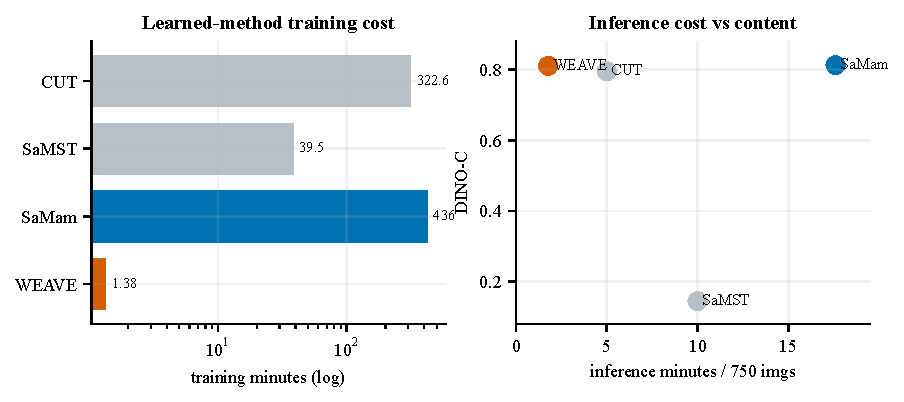
\includegraphics[width=0.82\textwidth]{supplement_figures/fig_cost_quality.pdf}
\caption{Cost accounting for learned baselines. WEAVE trains in minutes rather than
hundreds of minutes and remains in the high-content region at inference.}
\label{fig:supp-cost-quality}
\end{figure*}

\subsection{Baseline Data Inventory}

The baseline ledger contains both measured baselines and externally sourced or
API-limited methods. The evaluation convention is:
\begin{enumerate}
  \item collect generated images under a method/board/run directory;
  \item normalize filenames to the ordered source-target board;
  \item evaluate \clips{}, LPIPS, and optional side metrics using the shared evaluator;
  \item evaluate \dinos{} and \dinoc{} using the DINO sidecar scripts;
  \item record unavailable timings explicitly rather than estimating them from unrelated
  hardware.
\end{enumerate}

For D5-512, the paper table includes Identity, SD-Turbo, StyleAligned, Z-STAR,
StyleShot, CUT, SaMST, SaMam, Seedream 4.5, Latent-WCT, and WEAVE. For P2A-256 and
R5-WikiArt, the same naming convention is used, but some entries have fewer available
images or omitted timing fields. This is why each sidecar records image counts and skipped
counts rather than assuming all methods have a complete board.

\begin{center}
\footnotesize
\begin{tabularx}{\linewidth}{p{0.28\linewidth}p{0.27\linewidth}X}
\toprule
Method group & Output source & Notes \\
\midrule
Identity & evaluator no-op & Generated by copying/reading source image as output; defines style floor and content ceiling. \\
Latent-WCT & analytic transform & Zero trained parameters; evaluates whether wavelet statistics alone are sufficient. \\
CUT / SaMST / SaMam & learned baselines & SaMam is retrained on the same five-style D5 split as WEAVE and evaluated on the same 750 pairs; train/infer times measured on RTX~3060-class hardware when reported. \\
SD-Turbo / StyleAligned / Z-STAR / StyleShot & frozen-backbone editing baselines & Large pretrained backbones; no task-specific training counted, but inference wall-clock is reported when outputs were generated in the evaluation run. \\
Seedream 4.5 & API outputs & Parameter count and internal runtime are withheld; metrics are computed from saved outputs on the shared board. \\
WEAVE & single-RTX-3060 run & Main checkpoint and timing records come from the audited experiment tree. \\
\bottomrule
\end{tabularx}
\normalsize
\end{center}

\section{Ablation Summary}

The ablations support three complementary responsibilities: source-aligned endpoint
construction, learned LL/LH/HL residual transport, and stepwise analytic HF alignment.
Learned style memory provides a coarse registered-style prior rather than the main
image-specific style injector.

\begin{figure}[t]
\centering
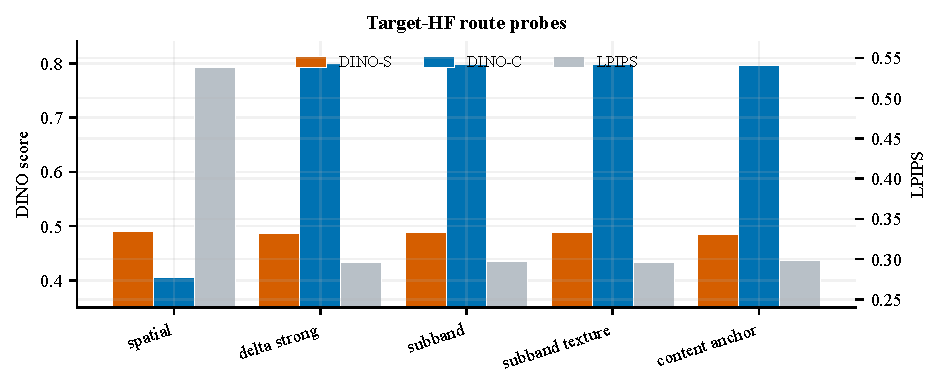
\includegraphics[width=0.9\linewidth]{supplement_figures/fig_probe_mechanisms.pdf}
\caption{Target-HF route ablation. Spatial target-HF injection raises style but
substantially reduces content scores, while pooled/subband target-HF routes preserve content at nearly the
same style level.}
\label{fig:supp-probe}
\end{figure}

The cross-attention branch is treated as auxiliary. Probe runs show near-closed gates
around 0.056--0.061 and weak gradient mass on the style-memory branch, yet the no-memory
subband run underperforms the standard subband route. The effective style movement comes
mainly from stepwise AdaIN/statistics, flow transport, and coordinate-free target-HF
codes; style memory supplies a useful coarse category prior but cannot replace the
image-specific HF route.

\paragraph{Analytic-alignment operator variants.}
The main model uses a single-level Haar decomposition and a global (channel-wise)
high-frequency alignment. We test two inference-time operator variants that keep the
trained field fixed: a \emph{two-level Haar} alignment (locks the coarser $\mathrm{LL}_2$
and aligns both Haar levels) and a \emph{block-local} HF alignment (per-$16\times16$
spatial-window mean/std matching instead of global). Both are applied at inference only,
so they add no parameters and negligible generation overhead. On the D5-750 board they
land within the baseline operating point: two-level Haar shifts slightly toward content
(DINO-C $0.819$ vs.\ $0.811$, LPIPS $0.256$ vs.\ $0.259$) at a small DINO-S cost, while
block-local HF raises CLIP-S ($0.718$ vs.\ $0.713$) but lowers DINO-C ($0.788$). Neither
improves the balanced point, supporting the single-level global design.

\begin{table}[t]
\centering
\small
\setlength{\tabcolsep}{4pt}
\begin{tabular}{@{}lccccr@{}}
\toprule
Variant & DINO-S$\uparrow$ & CLIP-S$\uparrow$ & LPIPS$\downarrow$ & DINO-C$\uparrow$ & Time (750) \\
\midrule
Single-level, global (main) & 0.4919 & 0.7128 & 0.2593 & 0.8107 & 88\,s \\
Two-level Haar & 0.4891 & 0.7110 & 0.2559 & 0.8186 & 79\,s \\
Block-local HF ($16^2$) & 0.4901 & 0.7185 & 0.2695 & 0.7878 & 83\,s \\
\bottomrule
\end{tabular}
\caption{Inference-time analytic-alignment operator variants on D5-750 (frozen D5
checkpoint, $\beta{=}2.0$, $\eta{=}0.1$, $K{=}8$). All are parameter-free operator
changes; generation time is per 750 pairs in PyTorch (the 73\,s/750 main figure uses
ONNX/TRT).}
\label{tab:supp-align-variants}
\end{table}

\subsection{Corrected Controls and Stability Checks}

The inference-time AdaIN control was rerun from the reported epoch-4 checkpoint after
verifying that the active nested configuration field was set to zero. All 20 checked
corresponding PNG hashes differ from the full model. Removing AdaIN changes DINO-S from
0.4916 to 0.4821 and CLIP-S from 0.7128 to 0.7005, while DINO-C increases from 0.8103 to
0.8455 and LPIPS decreases from 0.2593 to 0.2258. Thus the operator is active and induces
the intended style--content trade-off; the earlier no-effect result is not used.

For the matched training control, changing $\lambda_{LL}$ from 0.3 to 1.0 changes peak
DINO-S only from 0.4917 to 0.4910. The 1.0 run reaches its peak at epoch 3 and the frozen
probe selects epoch 5 with regret $6.8\times10^{-5}$. This supports robustness to a broad
nonzero LL weight, not a claim that 0.3 is uniquely optimal. In contrast, removing the
source-aligned endpoint yields peak DINO-S 0.4894 with LPIPS 0.3138, and the probe fires
eight epochs before that peak; this is the stronger endpoint-specific ablation.

Finally, reference-pool stability is evaluated without regenerating images. For each of
1,000 repetitions and each target style, one size-$m$ subset is sampled without replacement
from its 30 held-out references and reused for all 150 requests to that style. The board mean
of DINO-S(\weave{}) minus DINO-S(IDT) is positive in all repetitions: mean 0.0298 with
95\% interval [0.0204, 0.0394] for $m=8$, and mean 0.0319 with [0.0225, 0.0380] for
$m=16$. The corresponding per-request positive fractions are about 69\%, so this is
evidence for a stable board-level conclusion, not an assertion that every source improves.

\subsection{Alternative VAE Portability}

To test whether WEAVE depends on the SD1.5 EMA latent space, we replace its frozen VAE with
FLUX.1, FLUX.2, and Qwen-Image and retrain the wavelet-routed model. Only the latent-channel
projections are adapted to each VAE; the D5 data, one-level Haar routing, and evaluation
board are retained. This cross-VAE experiment uses the learned HH variant, whose
style--content trade-off is analyzed below.

\begin{table*}[t]
\centering
\small
\setlength{\tabcolsep}{5pt}
\begin{tabular}{@{}lcccccc@{}}
\toprule
Frozen VAE & Latent channels & Reported epoch & DINO-S$\uparrow$ & CLIP-S$\uparrow$ & LPIPS$\downarrow$ & DINO-C$\uparrow$ \\
\midrule
FLUX.1 & 16 & 6 & 0.4889 & 0.7134 & 0.2556 & 0.7801 \\
FLUX.2 & 32 & 29 & \textbf{0.4918} & \textbf{0.7165} & \textbf{0.2388} & \textbf{0.8728} \\
Qwen-Image & 16 & 1 & 0.4775 & 0.7144 & 0.2631 & 0.8251 \\
\bottomrule
\end{tabular}
\caption{Results after replacing the SD1.5 EMA VAE with recent frozen VAEs on D5. Each row
uses the same evaluation-free internal-dynamics selection protocol as the main SD1.5 run
(reported epoch is the selected training step under that rule).}
\label{tab:supp-vae-portability}
\end{table*}

The three VAEs all yield comparable style-transfer results, showing that WEAVE does not
depend on the older SD1.5 EMA representation and remains effective with newer VAE families.
The FLUX.2 run reaches the same DINO-S as the reported SD1.5 result while improving CLIP-S,
LPIPS, and DINO-C. Their optimization trajectories nevertheless differ: under the fixed
internal rule the selected epochs are 6 (FLUX.1), 29 (FLUX.2), and 1 (Qwen-Image). Frequency
routing transfers across tokenizers; the absolute gate/gradient threshold still shifts with
latent geometry, so cross-tokenizer early stopping benefits from per-tokenizer trajectory
normalization.

\paragraph{HH trade-off with a high-capacity VAE.}
On FLUX.2, increasing the HH velocity-loss weight from 0 to 20 changes DINO-S from 0.4911
to 0.4870 and CLIP-S from 0.6804 to 0.6740, while DINO-C rises from 0.8763 to 0.8888 and
LPIPS falls from 0.2359 to 0.2229. The intermediate weights follow the same trend. Learning
HH therefore provides a smooth content--style trade-off rather than a uniformly beneficial
or harmful route, consistent with retaining the simpler statistical HH treatment in the
main configuration.

\subsection{Frozen SD1.5 Extension}

We test whether the wavelet alignment operator transfers independently of the compact
velocity model. The control is a frozen SD1.5 image-to-image pipeline with an empty prompt,
strength 0.5, and 20 DDIM steps. The extension applies one-level Haar decomposition to the
output latent, aligns the channel-wise moments of LH, HL, and HH to the target-style latent
at scale 0.8, leaves LL unchanged, and then applies the inverse transform. No SD1.5 weights
are updated.

On the 600 cross-style D5 pairs, the base and extended editors obtain respectively
DINO-S 0.3974/0.4080, CLIP-S 0.7221/0.7366, LPIPS 0.3591/0.3630, and DINO-C
0.6589/0.6531. Both style gains are significant under paired $t$-tests
($p<10^{-15}$). On all 750 pairs, DINO-S changes from 0.4525 to 0.4613 and CLIP-S
from 0.7476 to 0.7594, while LPIPS remains 0.3586/0.3588 and DINO-C changes from
0.6583 to 0.6539. Timing over 720 completed requests gives 4.9\,ms per image for the
DWT--AdaIN--IDWT operation. The extension therefore isolates the portability of the
frequency-domain operator; it is not used to equate the compact model with SD1.5.



\section{Reproduction Commands}

Commands assume the minimal code package root as the working directory. Data and ONNX
graphs must be prepared locally (Section~\ref{sec:supp-onnx}).

\begin{lstlisting}[style=cmd,caption={Environment setup}]
python -m venv .venv
# activate .venv (Windows: .venv\Scripts\activate)
pip install torch torchvision --index-url https://download.pytorch.org/whl/cu128
pip install -r requirements.txt
# optional: pip install -r requirements-dev.txt  # pytest
\end{lstlisting}

\begin{lstlisting}[style=cmd,caption={Train the D5-512 paper checkpoint}]
# requires local data/train latents
python run.py --config configs/hf_oriented_internal_early_stop.json
\end{lstlisting}

\begin{lstlisting}[style=cmd,caption={Evaluate the selected D5 checkpoint (Table~1 D5 row)}]
python -m utils.run_evaluation \
  --checkpoint checkpoints/weave_epoch_0004.pt \
  --test_dir data/test \
  --output eval_outputs/d5_750_rerun \
  --config config.json \
  --config_override inference.json \
  --num_steps 8
\end{lstlisting}

\begin{lstlisting}[style=cmd,caption={Zero-shot diagnostic on R5 using the D5 checkpoint}]
# Does NOT reproduce the collection-specific R5 row in main-paper Table 1.
python -m utils.run_evaluation \
  --checkpoint checkpoints/weave_epoch_0004.pt \
  --test_dir data/images/r5/test \
  --output eval_outputs/r5_d5ckpt_zeroshot \
  --config config.json \
  --config_override inference.json \
  --num_steps 8
\end{lstlisting}

\begin{lstlisting}[style=cmd,caption={Generation-only timing (PyTorch fallback)}]
# Matches metric-free wall-clock protocol; the reported 73\,s figure uses ONNX/TRT
# (Section~\ref{sec:supp-onnx}), not this pure-PyTorch path.
python -m utils.run_evaluation \
  --checkpoint checkpoints/weave_epoch_0004.pt \
  --test_dir data/test \
  --output eval_outputs/timing \
  --config config.json \
  --config_override inference.json \
  --clip_backend none \
  --eval_disable_lpips \
  --num_steps 8 \
  --profile_timing \
  --force_regen
\end{lstlisting}

\subsection{End-to-End Checklist}

\begin{enumerate}[leftmargin=1.6em,itemsep=0.2em]
  \item Install the Python environment and confirm CUDA sees one RTX 3060-class GPU.
  \item Prepare local \path{data/train} and \path{data/test} (not in the minimal archive).
  \item Train with \path{configs/hf_oriented_internal_early_stop.json}, or use
  \path{checkpoints/weave_epoch_0004.pt}.
  \item Evaluate D5 with \texttt{inference.json} ($\beta{=}2.0$).
  \item Optionally export ONNX and compile TensorRT to match the 73.0\,s timing ledger.
  \item Treat R5/P2A Table~1 rows as collection-specific models not shipped in the minimal archive.
\end{enumerate}

\section{ONNX Export and TensorRT Compilation}
\label{sec:supp-onnx}

The reported 73.0\,s / 750 generation-only figure uses an optional accelerated VAE path.
\textbf{ONNX graphs and TensorRT engines are not included in the minimal anonymous archive}
because they exceed the package size budget ($\approx\!65$--$99$\,MB per graph). They can
be rebuilt from the public SD1.5 EMA VAE as follows.

\paragraph{Export.}
Encoder and decoder are exported separately with fixed batch size 8 (FP16) from the public
SD1.5 EMA VAE. WEAVE itself remains a PyTorch field; only the frozen VAE is exported. The
decoder latent scale \texttt{0.18215} is applied outside the ONNX graph. The minimal archive
does not include export utilities or ONNX binaries; the audited settings and stage-level
timing are documented in \path{docs/onnx_export_and_trt.md} for rebuilds.

\paragraph{TensorRT compile.}
Recommended: batch 8, FP16, workspace 2\,GB. On RTX 3060 12\,GB this compiles the decoder
in about 15 minutes and yields $\approx\!78.6$\,ms/image decode. Batch 16 requests
$\approx\!10.7$\,GB during build and OOMs on 12\,GB cards (engine falls back to weaker
tactics and can be slower). Workspace 4\,GB improves decode by only $\approx\!0.6\%$.

\paragraph{Pipeline timing (audited).}
With batch 8 and TRT workspace 2\,GB on one RTX 3060 12\,GB:
encoder$+$WEAVE 14.0\,s (18.7\,ms/image), TRT decoder 59.0\,s (78.6\,ms/image), total
\textbf{73.0\,s} (97.3\,ms/image; 10.3 pairs/s). Ledger:
\path{docs/generation_only_timing_summary.json}.

\section{Sanitized Artifact Ledger}

\begin{table*}[t]
\centering
\footnotesize
\caption{Artifacts for reproduction. Minimal archive contents vs.\ external requirements.}
\label{tab:supp-artifacts}
\begin{tabularx}{\textwidth}{p{0.34\textwidth}p{0.14\textwidth}X}
\toprule
Artifact & In archive? & Notes \\
\midrule
\path{configs/hf_oriented_internal_early_stop.json} & yes & D5 train config. \\
\path{config.json} / \path{inference.json} & yes & Base config; eval $\beta{=}2.0$ override. \\
\path{checkpoints/weave_epoch_0004.pt} & yes & Selected D5 checkpoint only. \\
\path{tools/prepare_submission_data.py} & yes & Path sanitize for local data. \\
\path{docs/generation_only_timing_summary.json} & yes & 73.0\,s timing ledger. \\
\path{docs/onnx_export_and_trt.md} & yes & ONNX/TRT rebuild protocol. \\
\path{data/README.md} & yes & Expected local data layout. \\
\path{data/train}, \path{data/test} & no & Prepare from WikiArt + VAE encode. \\
\path{data/onnx_exported/} & no & Export; not shipped (size). \\
P2A/R5 collection-specific checkpoints & no & Not required for D5 Table~1 row. \\
\bottomrule
\end{tabularx}
\normalsize
\end{table*}

\section{Known Limits}

The reported evidence supports a multi-objective operating point under automatic metrics
rather than universal dominance across metrics or datasets. The alternative-VAE experiments
establish compatibility with several recent latent representations, but do not establish
identical optimization dynamics, compute, or optimal stopping across tokenizers.

\end{document}
